\ifdefined\beamerclass
\else
  \def\beamerclass{beamer}
\fi

\ifdefined\articlemode
	\documentclass[]{article}
	\usepackage[a4paper,margin=2cm]{geometry}
	\usepackage[envcountsect]{beamerarticle}
	\usepackage{parskip}
	\usepackage[hidelinks]{hyperref}
\else
	 \documentclass[\beamerclass,ignorenonframetext]{beamer}
\fi


\usepackage{pgfpages}
\mode<handout>{
	% \setbeamercolor{background canvas}{bg=black!20}
	\pgfpagesuselayout{2 on 1}[a4paper,border shrink=5mm]
}

\usepackage{lmodern}
\usepackage{listings}
\usepackage{amsmath}
\usepackage{bm}
\usepackage{textpos} % package for the positioning

\usepackage{pgf, tikz}
\usetikzlibrary{arrows, automata}

\usetheme{Copenhagen}
\hypersetup{pdfstartview={Fit}}
\lstset{basicstyle=\small\ttfamily,breaklines=true}

\title[Automatic Differentiation]{Automatic Differentiation (Part I)}
\author{Jonathon Hare}
\institute[]
{
  Vision, Learning and Control\\
  University of Southampton 
}
\date{}
\subject{Computer Science}
\useoutertheme{infolines}
\setbeamertemplate{headline}{} %remove headline
\setbeamertemplate{navigation symbols}{} %remove navigation symbols

\definecolor{darkblue}{RGB}{37,55,97}
\definecolor{mellowyellow}{RGB}{247,206,70}
\definecolor{almostwhite}{RGB}{254,255,255}
\definecolor{merrygreen}{RGB}{79,173,91}
\definecolor{funkyorange}{RGB}{240,154,56}

\addtobeamertemplate{footnote}{\hskip -2em}{}
\newcommand\blfootnote[1]{%
  \begingroup
  \renewcommand\thefootnote{}\footnote{#1}%
  \addtocounter{footnote}{-1}%
  \endgroup
}

\begin{document}
\mode<article>{\maketitle}

\mode<presentation>{
\begin{frame}[plain]
        \begin{tikzpicture}[overlay, remember picture, shift={(current page.south west)},font={\fontfamily{Montserrat-TOsF}\selectfont}]
        \fill [merrygreen,text=darkblue] (0,0) rectangle (\paperwidth, \paperheight);
        \draw (4,7) node [align=left,text=almostwhite] {\Huge \begin{tabular}{l} \textbf{Differentiate} \\ \textbf{Automatically} \end{tabular}};
        \draw (11,1) node [align=left,text=almostwhite] {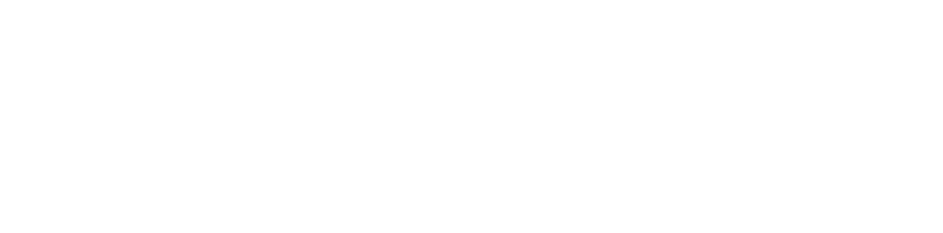
\includegraphics[scale=0.15]{../vlc.png}};
        \end{tikzpicture}
\end{frame}}

  \frame{
  \titlepage

\tiny{Much of this material is based on this blog post:
\url{https://rufflewind.com/2016-12-30/reverse-mode-automatic-differentiation}}
  }

\begin{frame}
\frametitle{What is Automatic Differentiation (AD)?}
To solve optimisation problems using gradient methods we need to compute the gradients (derivatives) of the objective with respect to the parameters.
\begin{itemize}
	\item In neural nets we're talking about the gradients of the loss function, $\mathcal{L}$ with respect to the parameters $\bm{\theta}$: 
	$\nabla_{\bm{\theta}} \mathcal{L} = \frac{\partial \mathcal{L}}{\partial \bm{\theta}}$
	\item AD is important - it's been suggested that ``Differentiable programming'' could be the term that ultimately replaces deep learning\footnote{\url{http://forums.fast.ai/t/differentiable-programming-is-this-why-we-switched-to-pytorch/9589/5}}.
\end{itemize}
\end{frame}

\begin{frame}
	\frametitle{How can you compute derivatives?}
There are three ways to compute derivatives:

% \begin{columns}
% 	\column{.45\textwidth}
%     \setbeamercovered{transparent}
%     \begin{itemize}
%     	\item<1,2> Symbolically differentiate the function with respect to its parameters
%     	\begin{itemize}
%     		\item by hand
%     		\item using a CAS
%     	\end{itemize}
%     	\item<1,3> Make estimates using finite differences
%     	\item<1,4> Use Automatic Differentiation
%     \end{itemize}

%     \column{.45\textwidth}
%       \begin{block}{Problems}<2>
%         Static - can't ``differentiate algorithms''
%       \end{block}
%       \begin{block}{Problems}<3>
%         Numerical errors - could compound in deep nets; expensive
%       \end{block}
%   \end{columns}
% \end{frame}

\begin{columns}
	\column{.45\textwidth}
    \setbeamercovered{transparent}
    \begin{itemize}
    	\item<1,2> Symbolically differentiate the function with respect to its parameters
    	\begin{itemize}
    		\item by hand
    		\item using a CAS
    	\end{itemize}
    	\item<1,3> Make estimates using finite differences
    	\item<1> Use Automatic Differentiation
    \end{itemize}

    \column{.45\textwidth}
      \begin{block}{Problems}<2>
        Static - can't ``differentiate algorithms''
      \end{block}
  \end{columns}
\end{frame}


\begin{frame}
		\frametitle{Numerical Differentiation}
	Suppose we can evaluate $f(x)$, but do not know how to differentiate it.

	\begin{block}{The basic idea}<2->
		Perturb the input by a small amount $h$, observe how much the output changes, and use the slope of the resulting secant line:
		\begin{equation*}
			f'(x) \approx \frac{f(x+h)-f(x)}{h}.
		\end{equation*}
	\end{block}

	\uncover<2->{This is a \textbf{one-sided finite difference}: it replaces a limit with two function evaluations at nearby points.}
\end{frame}


\begin{frame}
	\frametitle{What error have we introduced?}

	Taylor-expand $f(x+h)$ around $x$:
	\begin{align*}
		f(x+h) &= f(x) + h f'(x) + \frac{h^2}{2}f''(x) + O(h^3) \\[0.5em]
		\uncover<2->{\frac{f(x+h)-f(x)}{h}
		&= f'(x) + \frac{h}{2}f''(x) + O(h^2).}
	\end{align*}

	\begin{itemize}
		\item<3-> The first neglected term is proportional to $h$.
		\item<3-> We therefore say that the one-sided approximation has \textbf{truncation error} $O(h)$.
		\item<4-> Making $h$ smaller initially makes the estimate better.
	\end{itemize}
\end{frame}


\begin{frame}
	\frametitle{Using both sides cancels an error term}

	The \textbf{symmetric difference quotient} samples on both sides of $x$:
	\begin{equation*}
		f'(x) \approx \frac{f(x+h)-f(x-h)}{2h}.
	\end{equation*}

	\uncover<2->{Expanding both terms around $x$ gives}
	\begin{equation*}
		\uncover<2->{\frac{f(x+h)-f(x-h)}{2h}
		= f'(x) + \frac{h^2}{6}f'''(x) + O(h^4).}
	\end{equation*}

	\begin{itemize}
		\item<3-> The terms involving $f(x)$ and $f''(x)$ cancel.
		\item<4-> The truncation error is now $O(h^2)$ rather than $O(h)$.
		\item<5-> We spend one extra function evaluation to obtain a much better approximation for small $h$.
	\end{itemize}
\end{frame}


\begin{frame}
	\frametitle{Why not make $h$ as small as possible?}

	There are two competing sources of error:
	\begin{columns}
		\column{.46\textwidth}
		\begin{block}{Truncation error}<2->
			The finite difference is only an approximation to the limit.
			\begin{align*}
				\text{one-sided: } & O(h) \\
				\text{symmetric: } & O(h^2)
			\end{align*}
			It decreases as $h$ gets smaller.
		\end{block}

		\column{.46\textwidth}
		\begin{block}{Roundoff error}<3->
			The computer stores approximations to $x$, $x+h$ and the corresponding outputs.
			\begin{equation*}
				\text{error} \sim O\!\left(\frac{\epsilon_{\mathrm{mach}}}{h}\right)
			\end{equation*}
			It increases as $h$ gets smaller.
		\end{block}
	\end{columns}

	\uncover<4->{\centering There is a ``sweet spot'': too large truncates; too small rounds away the signal.}
\end{frame}


\begin{frame}
	\frametitle{Floating point numbers are not the reals}

	A floating point number has a finite number of bits for its sign, significand and exponent.

	\begin{itemize}
		\item Only a finite, non-uniformly spaced set of real numbers can be represented.
		\item The gap between adjacent representable values grows with the magnitude of the number.
		\item If $h$ is too small, the rounded value of $x+h$ can be exactly $x$.
		\item Even before that happens, subtracting the nearby values $f(x+h)$ and $f(x)$ discards shared leading digits: \textbf{catastrophic cancellation}.
	\end{itemize}

	\begin{block}{The consequence}<+->
		The numerator becomes dominated by rounding noise just as we try to make the mathematical approximation more accurate.
	\end{block}
\end{frame}


\begin{frame}
	\frametitle{Numerical differentiation needs double precision}

	\begin{columns}
		\column{.45\textwidth}
		\begin{block}{32-bit floating point}<1->
			\begin{itemize}
				\item about 7 decimal digits
				\item $\epsilon_{\mathrm{mach}} \approx 1.2\times10^{-7}$
			\end{itemize}
		\end{block}

		\column{.45\textwidth}
		\begin{block}{64-bit floating point}<2->
			\begin{itemize}
				\item about 16 decimal digits
				\item $\epsilon_{\mathrm{mach}} \approx 2.2\times10^{-16}$
			\end{itemize}
		\end{block}
	\end{columns}

	\begin{itemize}
		\item<3-> A rough choice for symmetric differences is $h\sim\sqrt[3]{\epsilon_{\mathrm{mach}}}$, although the best value also depends on the scale and curvature of $f$.
		\item<4-> Single precision leaves very little room between truncation and roundoff error; half precision is worse still.
		\item<5-> For gradient checking, evaluate both the function and the gradients in \textbf{double precision}.
	\end{itemize}
	\blfootnote{PyTorch numerical accuracy notes: \url{https://docs.pytorch.org/docs/stable/notes/numerical_accuracy.html}}
\end{frame}


\begin{frame}
	\frametitle{Finite differences do not scale to training}

	Let $\mathcal{L}:\mathbb{R}^p\rightarrow\mathbb{R}$ be a loss with $p$ parameters.

	\begin{itemize}
		\item A one-sided numerical gradient needs $p+1$ evaluations of $\mathcal{L}$.
		\item A symmetric numerical gradient needs $2p$ evaluations.
		\item A model with millions of parameters would therefore need millions of forward passes for \emph{one} gradient step.
		\item The estimates also contain truncation and roundoff error.
	\end{itemize}

	\begin{alertblock}{So why learn this?}<+->
		A slow, independent approximation is extremely useful for checking whether a fast derivative implementation is correct.
	\end{alertblock}
\end{frame}


\begin{frame}[fragile]
	\frametitle{Finite differences make good gradient checks}

	For a scalar loss, compare an AD gradient $g_{\mathrm{AD}}$ with a symmetric finite-difference estimate $g_{\mathrm{FD}}$:
	\begin{equation*}
		\frac{\lVert g_{\mathrm{AD}}-g_{\mathrm{FD}}\rVert}
		{\max\!\left(1,\lVert g_{\mathrm{AD}}\rVert,\lVert g_{\mathrm{FD}}\rVert\right)}.
	\end{equation*}

	\begin{columns}
		\column{.55\textwidth}
		\begin{itemize}
			\item Use double precision.
			\item Make the computation deterministic.
			\item Avoid non-differentiable test points.
			\item Check a few coordinates or directions for very large models.
		\end{itemize}

		\column{.40\textwidth}
		\begin{lstlisting}[basicstyle=\tiny\ttfamily]
import torch.autograd as ag

x = x.double()
x.requires_grad_()
ag.gradcheck(f, (x,))
		\end{lstlisting}
	\end{columns}
	\blfootnote{\url{https://docs.pytorch.org/docs/stable/generated/torch.autograd.gradcheck.gradcheck.html}}
\end{frame}

\begin{frame}
	\frametitle{How can you compute derivatives?}
There are three ways to compute derivatives:

\begin{columns}
	\column{.45\textwidth}
    \setbeamercovered{transparent}
    \begin{itemize}
    	\item<0> Symbolically differentiate the function with respect to its parameters
    	\begin{itemize}
    		\item by hand
    		\item using a CAS
    	\end{itemize}
    	\item<1> Make estimates using finite differences
    	\item<2> Use Automatic Differentiation
    \end{itemize}

    \column{.45\textwidth}
      \begin{block}{Problems}<1>
        Numerical errors - could compound in deep nets; expensive
      \end{block}
  \end{columns}
\end{frame}

\begin{frame}
	\frametitle{What is Automatic Differentiation (AD)?}

	Automatic Differentiation is:
	\begin{itemize}
		\item a method to get exact derivatives efficiently, by storing information as you go forward that you can reuse as you go backwards.
		\begin{itemize}
			\item Takes code that computes a function and uses that to compute the derivative of that function.
		\item The goal isn't to obtain closed-form solutions, but to be able to write a program that efficiently computes the derivatives.
		\end{itemize}
	\end{itemize}
\end{frame}

\begin{frame}[fragile]
\frametitle{Lets think about differentiation and programming}
\begin{columns}
	\column{.45\textwidth}
    \begin{example}<1->[Math] 
    \vspace{-1.5em}
    \begin{align*}
			x & = ? \\
			y & = ? \\
			a & = x \, y \\
			b & = \sin(x) \\
			z & = a + b
		\end{align*}
    \end{example}

	\column{.45\textwidth}
	\begin{example}<2->[Code]
			\begin{lstlisting}
x = ?
y = ?
a = x * y
b = sin(x)
z = a + b
			\end{lstlisting}
	\end{example}
	\end{columns}
\end{frame}

\begin{frame}
\frametitle{The Chain Rule of Differentiation}

\uncover<1->{
Recall the chain rule for a variable/function $z$ that depends on $y$ which depends on $x$:
\begin{equation*}
\frac{dz}{dx} = \frac{dz}{dy}\frac{dy}{dx}
\end{equation*}
}

\uncover<2->{
In general, the chain rule can be expressed as:
\begin{equation*}
	\frac{\partial w}{\partial t} = \sum_i^N \frac{\partial w}{\partial u_i} \frac{\partial u_i}{\partial t} = \frac{\partial w}{\partial u_1}\frac{\partial u_1}{\partial t} + \frac{\partial w}{\partial u_2}\frac{\partial u_2}{\partial t} + \dots + \frac{\partial w}{\partial u_N}\frac{\partial u_N}{\partial t}
\end{equation*}
where $w$ is some output variable, and $u_i$ denotes each input variable $w$ depends on.
}
\end{frame}

\begin{frame}
\frametitle{Applying the Chain Rule}

Let's differentiate our previous expression with respect to some yet to be given variable $t$:
\begin{columns}
\column{.3\textwidth}
\begin{block}<1->{Expression}
    \vspace{-1.5em}
    \begin{align*}
			x & = ? \\
			y & = ? \\
			a & = x \, y \\
			b & = \sin(x) \\
			z & = a + b
		\end{align*}
    \end{block}

\column{.65\textwidth}
\begin{align*}
	\frac{\partial x}{\partial t} & = ? \\
	\frac{\partial y}{\partial t} & = ? \\
	\frac{\partial a}{\partial t} & = x \frac{\partial y}{\partial t} + y \frac{\partial x}{\partial t}\\
	\frac{\partial b}{\partial t} & = \cos(x) \frac{\partial x}{\partial t}\\
	\frac{\partial z}{\partial t} & = \frac{\partial a}{\partial t} + \frac{\partial b}{\partial t}
\end{align*}
\end{columns}
\vfill
 
\uncover<2->{If we substitute $t=x$ in the above we'll have an algorithm for computing $\partial z/\partial x$. To get $\partial z/\partial y$ we'd just substitute $t=y$.
}

\end{frame}

\begin{frame}[fragile]
\frametitle{Translating to code I}
We could translate the previous expressions back into a program involving \emph{differential variables} \lstinline!{dx, dy, ...}! which represent $\partial x/\partial t, \partial y/\partial t, \dots$ respectively:

\begin{lstlisting}
dx = ?
dy = ?
da = y * dx + x * dy
db = cos(x) * dx
dz = da + db	
\end{lstlisting}

\uncover<2->{What happens to this program if we substitute $t=x$ into the math expression?}
\end{frame}

\begin{frame}[fragile]
\frametitle{Translating to code II}

\begin{columns}
\column{.45\textwidth}
\begin{lstlisting}
dx = 1
dy = 0
da = y * dx + x * dy
db = cos(x) * dx
dz = da + db	
\end{lstlisting}

\column{.45\textwidth}

\uncover<2->{The effect is remarkably simple: to compute $\partial z/\partial x$ we just seed the algorithm with \lstinline!dx=1! and \lstinline!dy=0!.}
\end{columns}
\end{frame}


\begin{frame}[fragile]
\frametitle{Translating to code III}

\begin{columns}
\column{.45\textwidth}
\begin{lstlisting}
dx = 0
dy = 1
da = y * dx + x * dy
db = cos(x) * dx
dz = da + db	
\end{lstlisting}

\column{.45\textwidth}

To compute $\partial z/\partial y$ we just seed the algorithm with \lstinline!dx=0! and \lstinline!dy=1!.
\end{columns}
\end{frame}

\begin{frame}[fragile]
\frametitle{Making Rules}

\begin{itemize}
	\item<+-> We've successfully computed the gradients for a specific function, but the process was far from automatic. 
	\item<+-> We need to formalise a set of rules for translating a program that evaluates an expression into a program that evaluates its derivatives.
	\item<+-> We have actually already discovered 3 of these rules:
\begin{lstlisting}
c = a + b   =>  dc = da + db
c = a * b   =>  dc = b * da + a * db
c = sin(a)  =>  dc = cos(a) * da
\end{lstlisting}
\end{itemize}

\end{frame}

\begin{frame}[fragile]
\frametitle{More rules}

These initial rules:
\begin{lstlisting}
c=a+b     =>  dc=da+db
c=a*b     =>  dc=b*da+a*db
c=sin(a)  =>  dc=cos(a)*da
\end{lstlisting}
can easily be extended further using multivariable calculus:
\begin{lstlisting}
c=a-b     =>  dc=da-db
c=a/b     =>  dc=da/b-a*db/b**2
c=a**b    =>  dc=b*a**(b-1)*da+log(a)*a**b*db
c=cos(a)  =>  dc=-sin(a)*da
c=tan(a)  =>  dc=da/cos(a)**2
\end{lstlisting}
\end{frame}

\begin{frame}
\frametitle{Forward Mode AD}
\begin{itemize}
	\item<+-> To translate using the rules we simply replace each primitive operation in the original program by its differential analogue.
	\item<+-> The order of computation remains unchanged: if a statement $K$ is evaluated before another statement $L$, then the differential analogue of $K$ is evaluated before the analogue statement of $L$.
	\item<+-> This is \textbf{Forward-mode Automatic Differentiation}.
\end{itemize}
\end{frame}

\begin{frame}[fragile]
\frametitle{Interleaving differential computation}

A careful analysis of our original program and its differential analogue shows that its possible to interleave the differential calculations with the original ones:
\begin{columns}
	\column{.45\textwidth}
\begin{lstlisting}
x  = ?
dx = ?

y  = ?
dy = ?

a  = x * y
da = y * dx + x * dy

b  = sin(x)
db = cos(x) * dx

z  = a + b
dz = da + db
\end{lstlisting}

\column{.45\textwidth}
\begin{block}{Dual Numbers}<2->
	\begin{itemize}
		\item<2-> This implies that we can keep track of the value and gradient at the same time.
		\item<3-> We can use a mathematical concept called a ``Dual Number'' to create a very simple direct implementation of AD.
	\end{itemize}
\end{block}

\end{columns}
\end{frame}


\begin{frame}
\frametitle{Forward mode computes a JVP}

For a function $\bm{f}:\mathbb{R}^n\rightarrow\mathbb{R}^m$, carry an input value and an input tangent together:
\begin{equation*}
	(\bm{x},\dot{\bm{x}}) \longmapsto
	\left(\bm{f}(\bm{x}),\dot{\bm{y}}\right),
	\qquad
	\dot{\bm{y}} = \bm{J}_{\bm{f}}(\bm{x})\dot{\bm{x}}.
\end{equation*}

\begin{itemize}
	\item<2-> The propagated tangent $\dot{\bm{y}}$ is a \textbf{Jacobian-vector product} (JVP).
	\item<3-> Choosing $\dot{\bm{x}}=\bm{e}_i$ gives the $i$th column of the Jacobian ($\bm{e}_i$ is the i-th standard basis vector).
	\item<4-> Choosing an arbitrary $\dot{\bm{x}}=\bm{v}$ gives the change in the output in direction $\bm{v}$, without constructing the Jacobian.
\end{itemize}
\end{frame}


\begin{frame}
\frametitle{The JVP is a directional derivative}

The JVP has an equivalent limit definition:
\begin{equation*}
	\bm{J}_{\bm{f}}(\bm{x})\bm{v}
	=
	\left.\frac{d}{dt}\bm{f}(\bm{x}+t\bm{v})\right|_{t=0}.
\end{equation*}

\uncover<2->{We could approximate it numerically:}
\begin{equation*}
	\uncover<2->{\bm{J}_{\bm{f}}(\bm{x})\bm{v}
	\approx
	\frac{\bm{f}(\bm{x}+h\bm{v})-\bm{f}(\bm{x}-h\bm{v})}{2h}.}
\end{equation*}

\begin{block}{Forward mode does something better}<3->
	It propagates the same directional derivative through every primitive operation using the chain rule---accurate to floating point precision, with no choice of $h$.
\end{block}
\end{frame}


\begin{frame}[fragile]
\frametitle{Computing a JVP with PyTorch}

\begin{lstlisting}
import torch
from torch.func import jvp

def f(x):
    return torch.stack((x[0] * x[1], torch.sin(x[0])))

x = torch.tensor([2., 3.], dtype=torch.double)
v = torch.tensor([1., 0.], dtype=torch.double)

y, Jv = jvp(f, (x,), (v,))
\end{lstlisting}

\begin{itemize}
	\item<2-> \texttt{y} is $\bm{f}(\bm{x})$.
	\item<3-> \texttt{Jv} is $\bm{J}_{\bm{f}}(\bm{x})\bm{v}$; here it is $[3,\cos(2)]^\top$.
	\item<4-> Each primal input has a tangent with the same shape.
\end{itemize}
\blfootnote{\url{https://docs.pytorch.org/docs/stable/generated/torch.func.jvp.html}}
\end{frame}


\begin{frame}[fragile]
\frametitle{PyTorch also exposes the dual tensors}

The lower-level API makes the mechanism explicit:
\begin{lstlisting}
from torch.autograd import forward_ad as fwAD

with fwAD.dual_level():
    dual_x = fwAD.make_dual(x, v)
    dual_y = f(dual_x)
    y, Jv = fwAD.unpack_dual(dual_y)
\end{lstlisting}

\begin{itemize}
	\item<2-> \texttt{make\_dual} pairs the primal $\bm{x}$ with the tangent $\bm{v}$.
	\item<3-> Ordinary PyTorch operations propagate both components.
	\item<4-> \texttt{unpack\_dual} separates the output value from its JVP.
\end{itemize}

\uncover<5->{For routine JVPs, prefer the higher-level \texttt{torch.func.jvp}; the dual-tensor API is useful when you need finer control.}
\blfootnote{\url{https://docs.pytorch.org/tutorials/intermediate/forward_ad_usage.html}}
\end{frame}



\end{document}
